\documentclass[conference]{IEEEtran}

\usepackage{graphicx}
\usepackage{booktabs}

\title{Performance Analysis of OpenMP Runtime Parameters for Parallel Pi Approximation}

\author{
\IEEEauthorblockN{Anwith Goud Ganamaina}
\IEEEauthorblockA{Department of Computer Science\\
Texas State University\\
San Marcos, TX, USA}
}

\begin{document}

\maketitle

\begin{abstract}
This project analyzes the performance of an OpenMP parallel program that approximates the value of Pi using numerical integration. Experiments were conducted on the Lonestar6 high performance computing system to evaluate the effect of different OpenMP runtime parameters including thread placement, number of threads, and scheduling policies. The results demonstrate that proper thread placement and scheduling strategies significantly influence program performance.
\end{abstract}

\section{Introduction}

Parallel computing allows computational tasks to be executed simultaneously using multiple processor cores. OpenMP is a shared-memory parallel programming model that enables developers to parallelize applications using compiler directives. In this assignment, a serial program that approximates the value of Pi was parallelized using OpenMP. The objective of this project was to study how OpenMP runtime parameters influence performance on the Lonestar6 supercomputer.

\section{Task 1: System Architecture using hwloc}

The architecture of the Lonestar6 compute node was analyzed using the hwloc tool. The hwloc utility provides detailed information about the hardware topology including sockets, cores, cache levels, and memory.

Ideally the command used is:

\begin{verbatim}
lstopo --no-io
\end{verbatim}

This command reveals the hierarchical structure of the compute node. The system consists of multiple CPU sockets with several cores per socket. Each core has private L1 and L2 caches while an L3 cache is shared among cores within a socket. The node also provides a large shared memory space available to all threads. Understanding this architecture is important when selecting OpenMP thread placement policies such as OMP\_PLACES and OMP\_PROC\_BIND.

\section{OpenMP Implementation}

The serial program was parallelized using the following OpenMP directive:

\begin{verbatim}
#pragma omp parallel for reduction(+:sum) schedule(runtime)
\end{verbatim}

The parallel for directive distributes loop iterations across multiple threads. The reduction clause ensures that each thread maintains a private copy of the variable sum and safely combines partial results at the end of execution. The schedule(runtime) clause allows scheduling policies to be modified using environment variables without recompiling the program.

\begin{table}[htbp]
\caption{OpenMP Variable Scope}
\centering
\begin{tabular}{ll}
\toprule
Variable & Scope \\
\midrule
sum & reduction variable \\
i & private \\
x & private \\
step & shared \\
num\_steps & shared \\
\bottomrule
\end{tabular}
\end{table}

\section{Thread Placement Performance}

Different thread placement configurations were tested using the OpenMP environment variables OMP\_PLACES and OMP\_PROC\_BIND. The results are shown in Table II.

\begin{table}[htbp]
\caption{Thread Placement Results}
\centering
\begin{tabular}{lll}
\toprule
OMP\_PLACES & OMP\_PROC\_BIND & Time (s) \\
\midrule
core & close & 0.003335 \\
core & spread & 0.002798 \\
socket & close & 0.002630 \\
socket & spread & 0.002743 \\
\bottomrule
\end{tabular}
\end{table}

\begin{figure}[htbp]
\centering
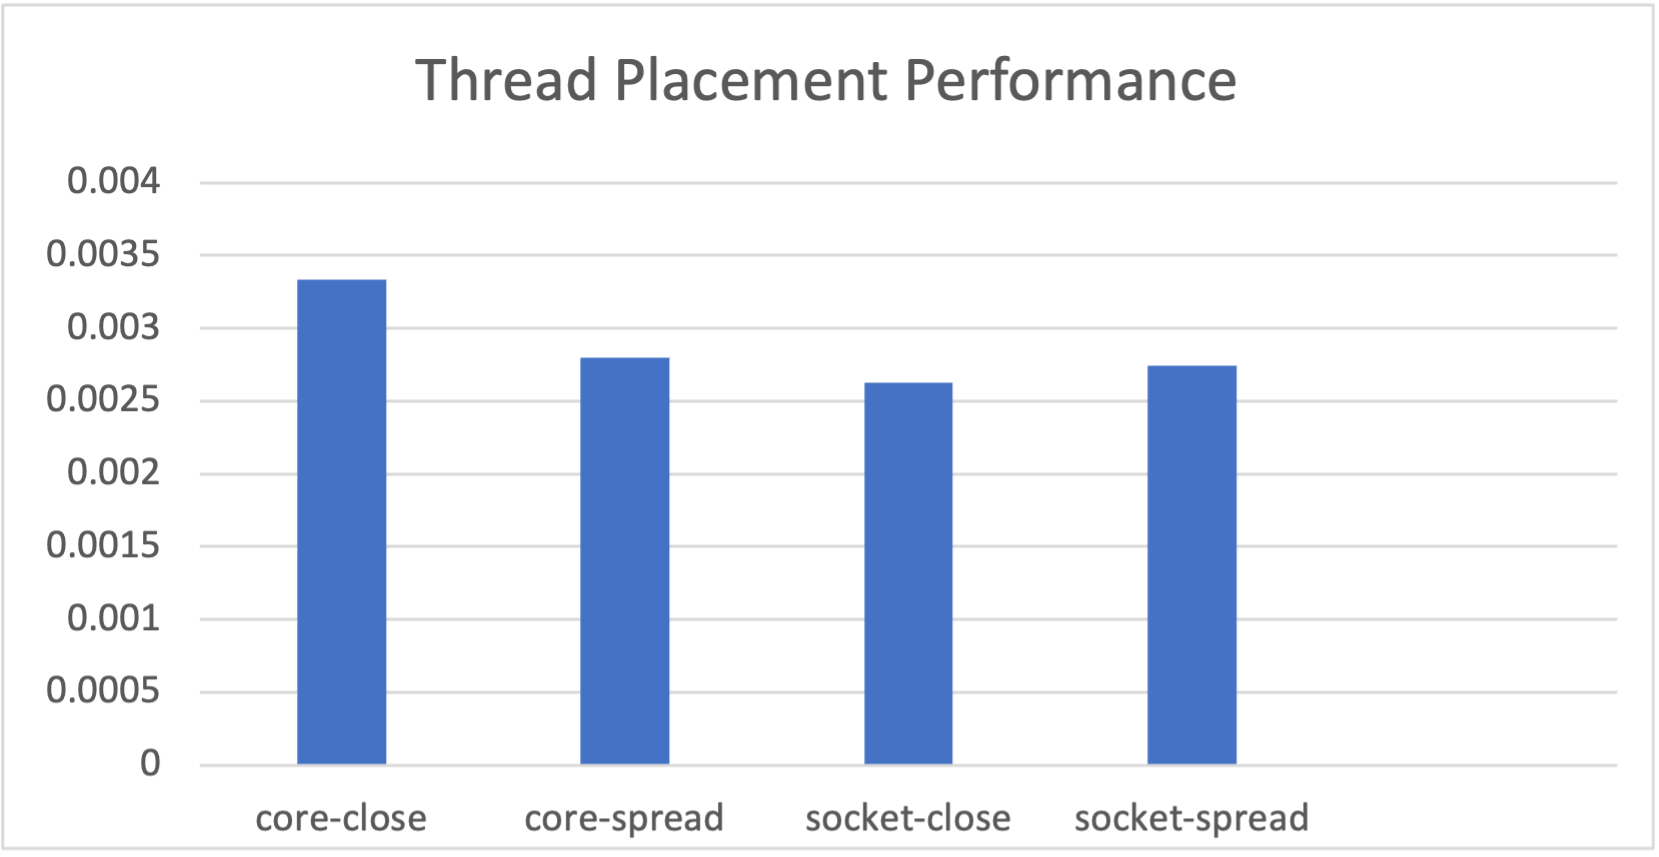
\includegraphics[width=0.45\textwidth]{placement.png}
\caption{Thread placement performance comparison}
\end{figure}

\section{Thread Scaling Performance}

The program was executed using different numbers of threads to observe how performance scales with increasing parallelism.

\begin{figure}[htbp]
\centering
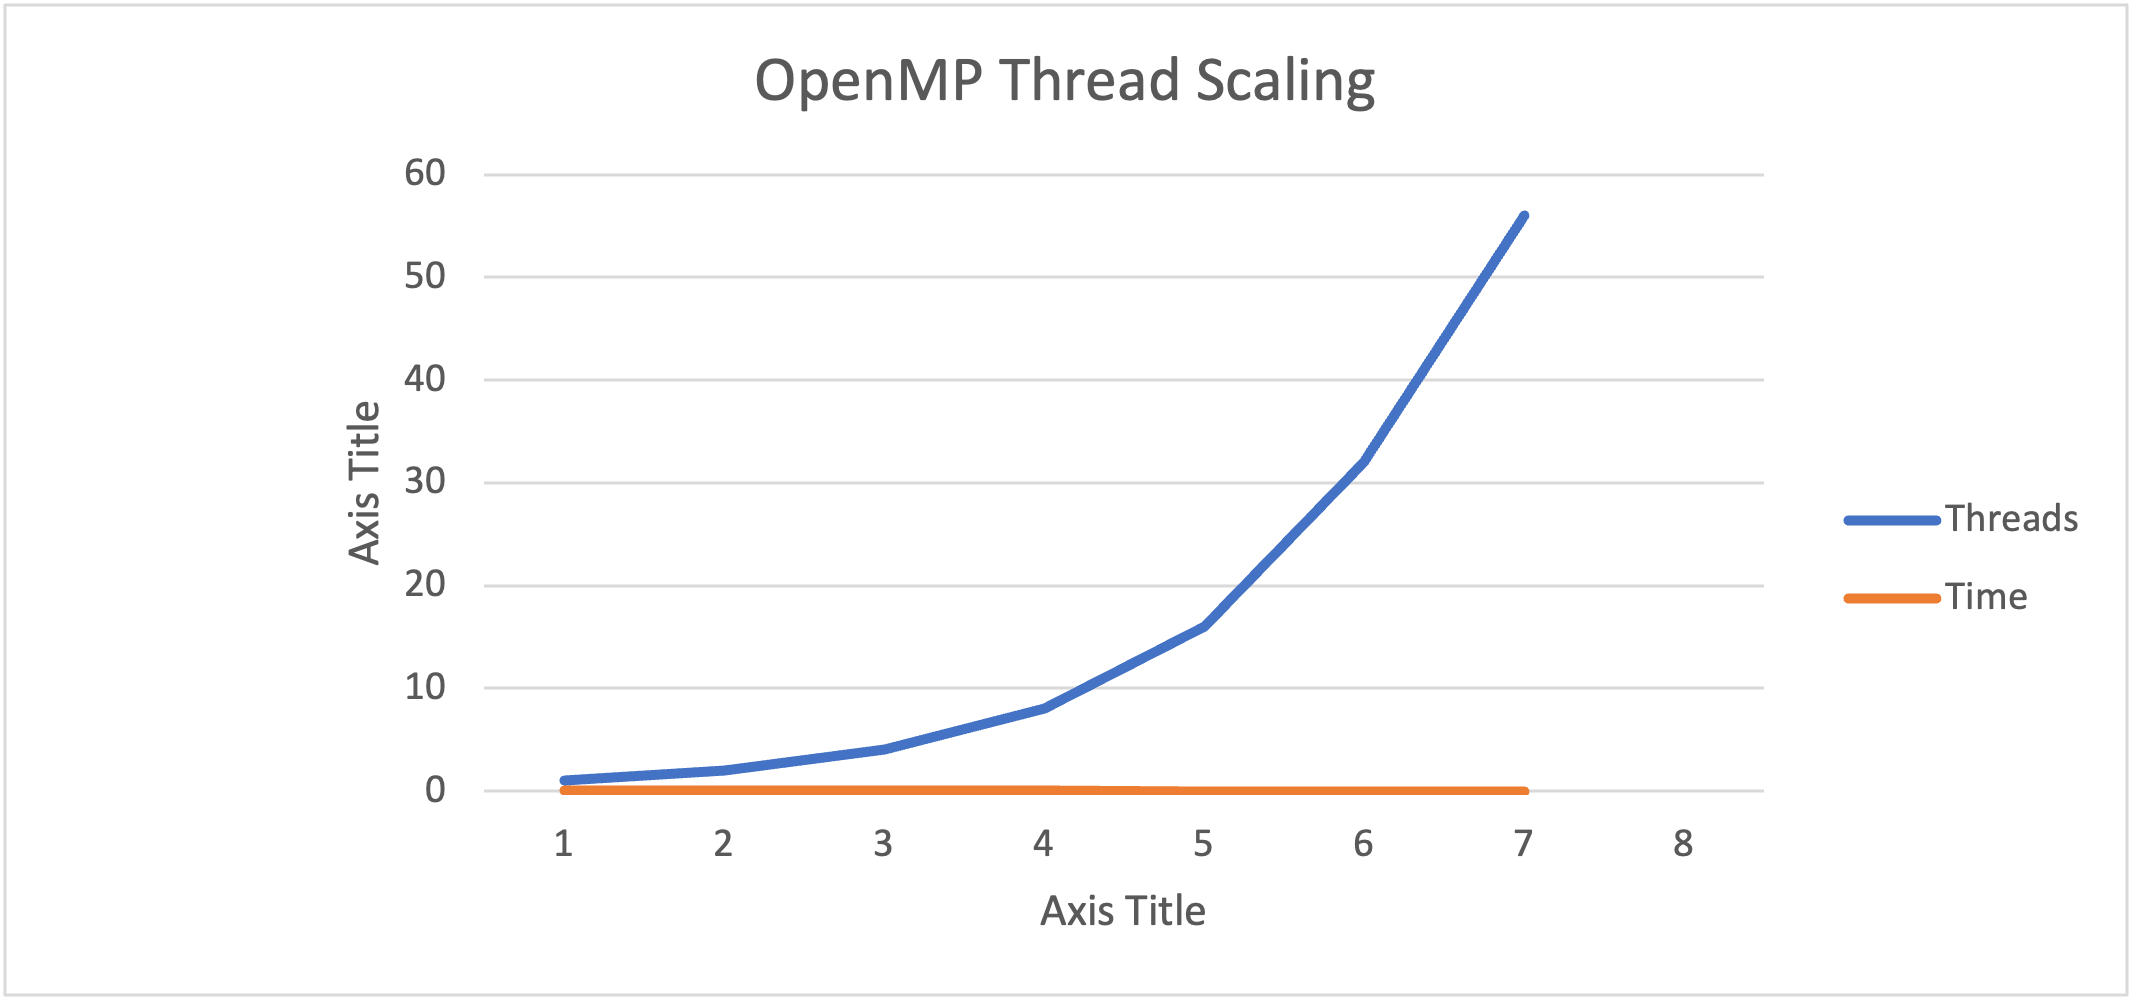
\includegraphics[width=0.45\textwidth]{scaling.png}
\caption{OpenMP thread scaling performance}
\end{figure}

The results show that execution time decreases as the number of threads increases because the workload is distributed among multiple processor cores. However, the improvement becomes smaller as the number of threads approaches the maximum number of cores available on the node.

\section{Scheduling Policy Performance}

Different scheduling policies were tested to determine how OpenMP distributes loop iterations across threads.

\begin{table}[htbp]
\caption{Scheduling Policy Results}
\centering
\begin{tabular}{lc}
\toprule
Schedule Policy & Time (s) \\
\midrule
static,10 & 0.001291 \\
static,100 & 0.001236 \\
static,1000 & 0.001261 \\
dynamic,10 & 0.029048 \\
dynamic,100 & 0.003799 \\
dynamic,1000 & 0.001623 \\
\bottomrule
\end{tabular}
\end{table}

\begin{figure}[htbp]
\centering
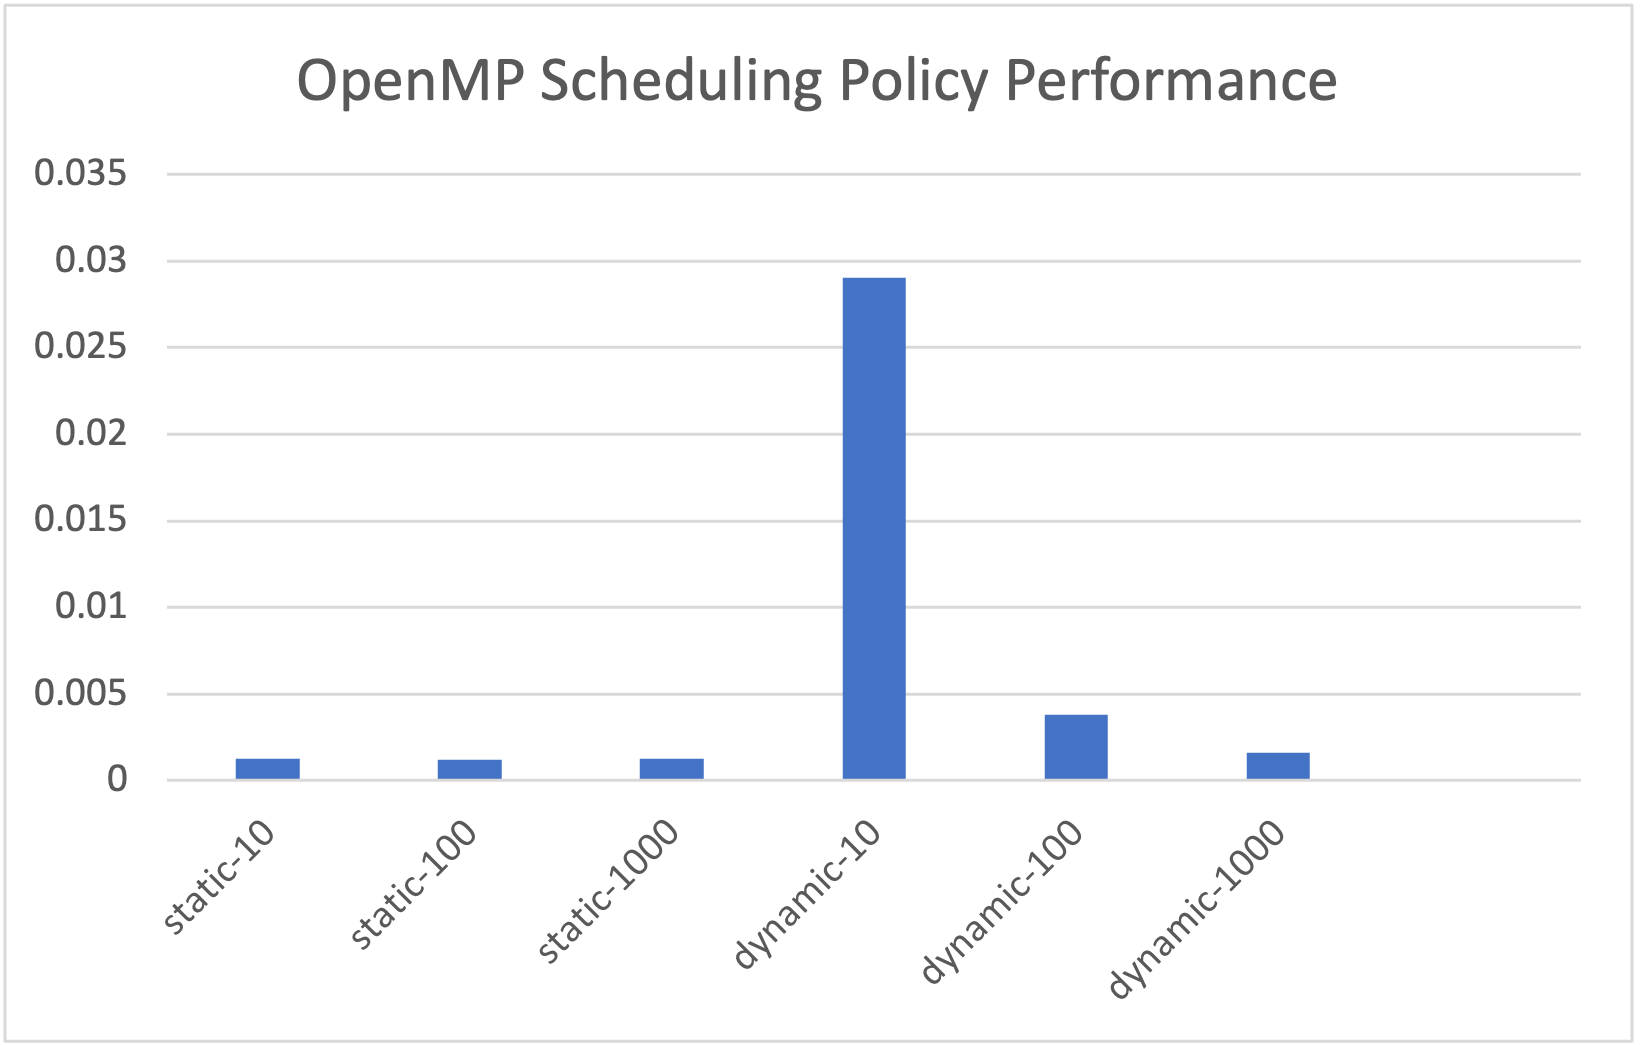
\includegraphics[width=0.45\textwidth]{schedule.png}
\caption{Scheduling policy performance comparison}
\end{figure}

\section{Conclusion}

This project demonstrated how OpenMP runtime parameters affect the performance of parallel programs on high performance computing systems. Experiments showed that thread placement, number of threads, and scheduling policies significantly influence execution time. The best performance was achieved when threads were placed across sockets with close binding and when static scheduling with moderate chunk sizes was used. These results highlight the importance of understanding hardware architecture and runtime configuration when optimizing parallel applications.

\end{document}
